\documentclass[11 pt]{article}
\usepackage{graphicx}
\title{
	Design suitable exchange of messages allowing a fair match between two opponents \\
	\large HW6 - CNS Sapienza}
\author{Luigi Russo 1699981}
\date{7/12/2018}

\begin{document}

\maketitle

\section{Goals}
The goal of this homework is to define a protocol in order to allow two parties (Alice and Bob) to play a fair match. In particular we should:
\begin{itemize}
	\item enforce data integrity
	\item prevent players from obtaining \textbf{unfair} advantage from pre-computation
	\item contrast replay attacks
\end{itemize}
Moreover it is allowed to use (\textbf{but not all of them!}) nonces, timestamps, hash functions, symmetric encryption / decryption, public key cryptography, and so on.
The protocol should be also as simple as possible, providing the same guarantees the analogical players have.

\section{Rules}
A match is a sequence of N roshambo games, where N = 2p + 1. Each player aims to win the match and in order to do it, he has to win at least p + 1 games. There are only three possible choices: "Paper" ,"Rock" and "Scissors". Users can't see each other, they use smartphones to exchange messages. Even if there are no trusted authorities nor third parties and each user does not trust the other one, everyone respects the game protocol (a precise sequence of messages). Any dispute regarding the winner of a game or the winner of a match should be prevented. Users will cheat if there is the possibility to cheat without being discovered (a weak protocol!)

\section{Protocol}
This is the protocol that I have designed. I have assumed that N is a constant number. I have only used nonces and a cryptographic hash function H, so no symmetric (or asymmetric) encryptions and no timestamps.

\begin{figure}[!ht]
	\centering % optional
	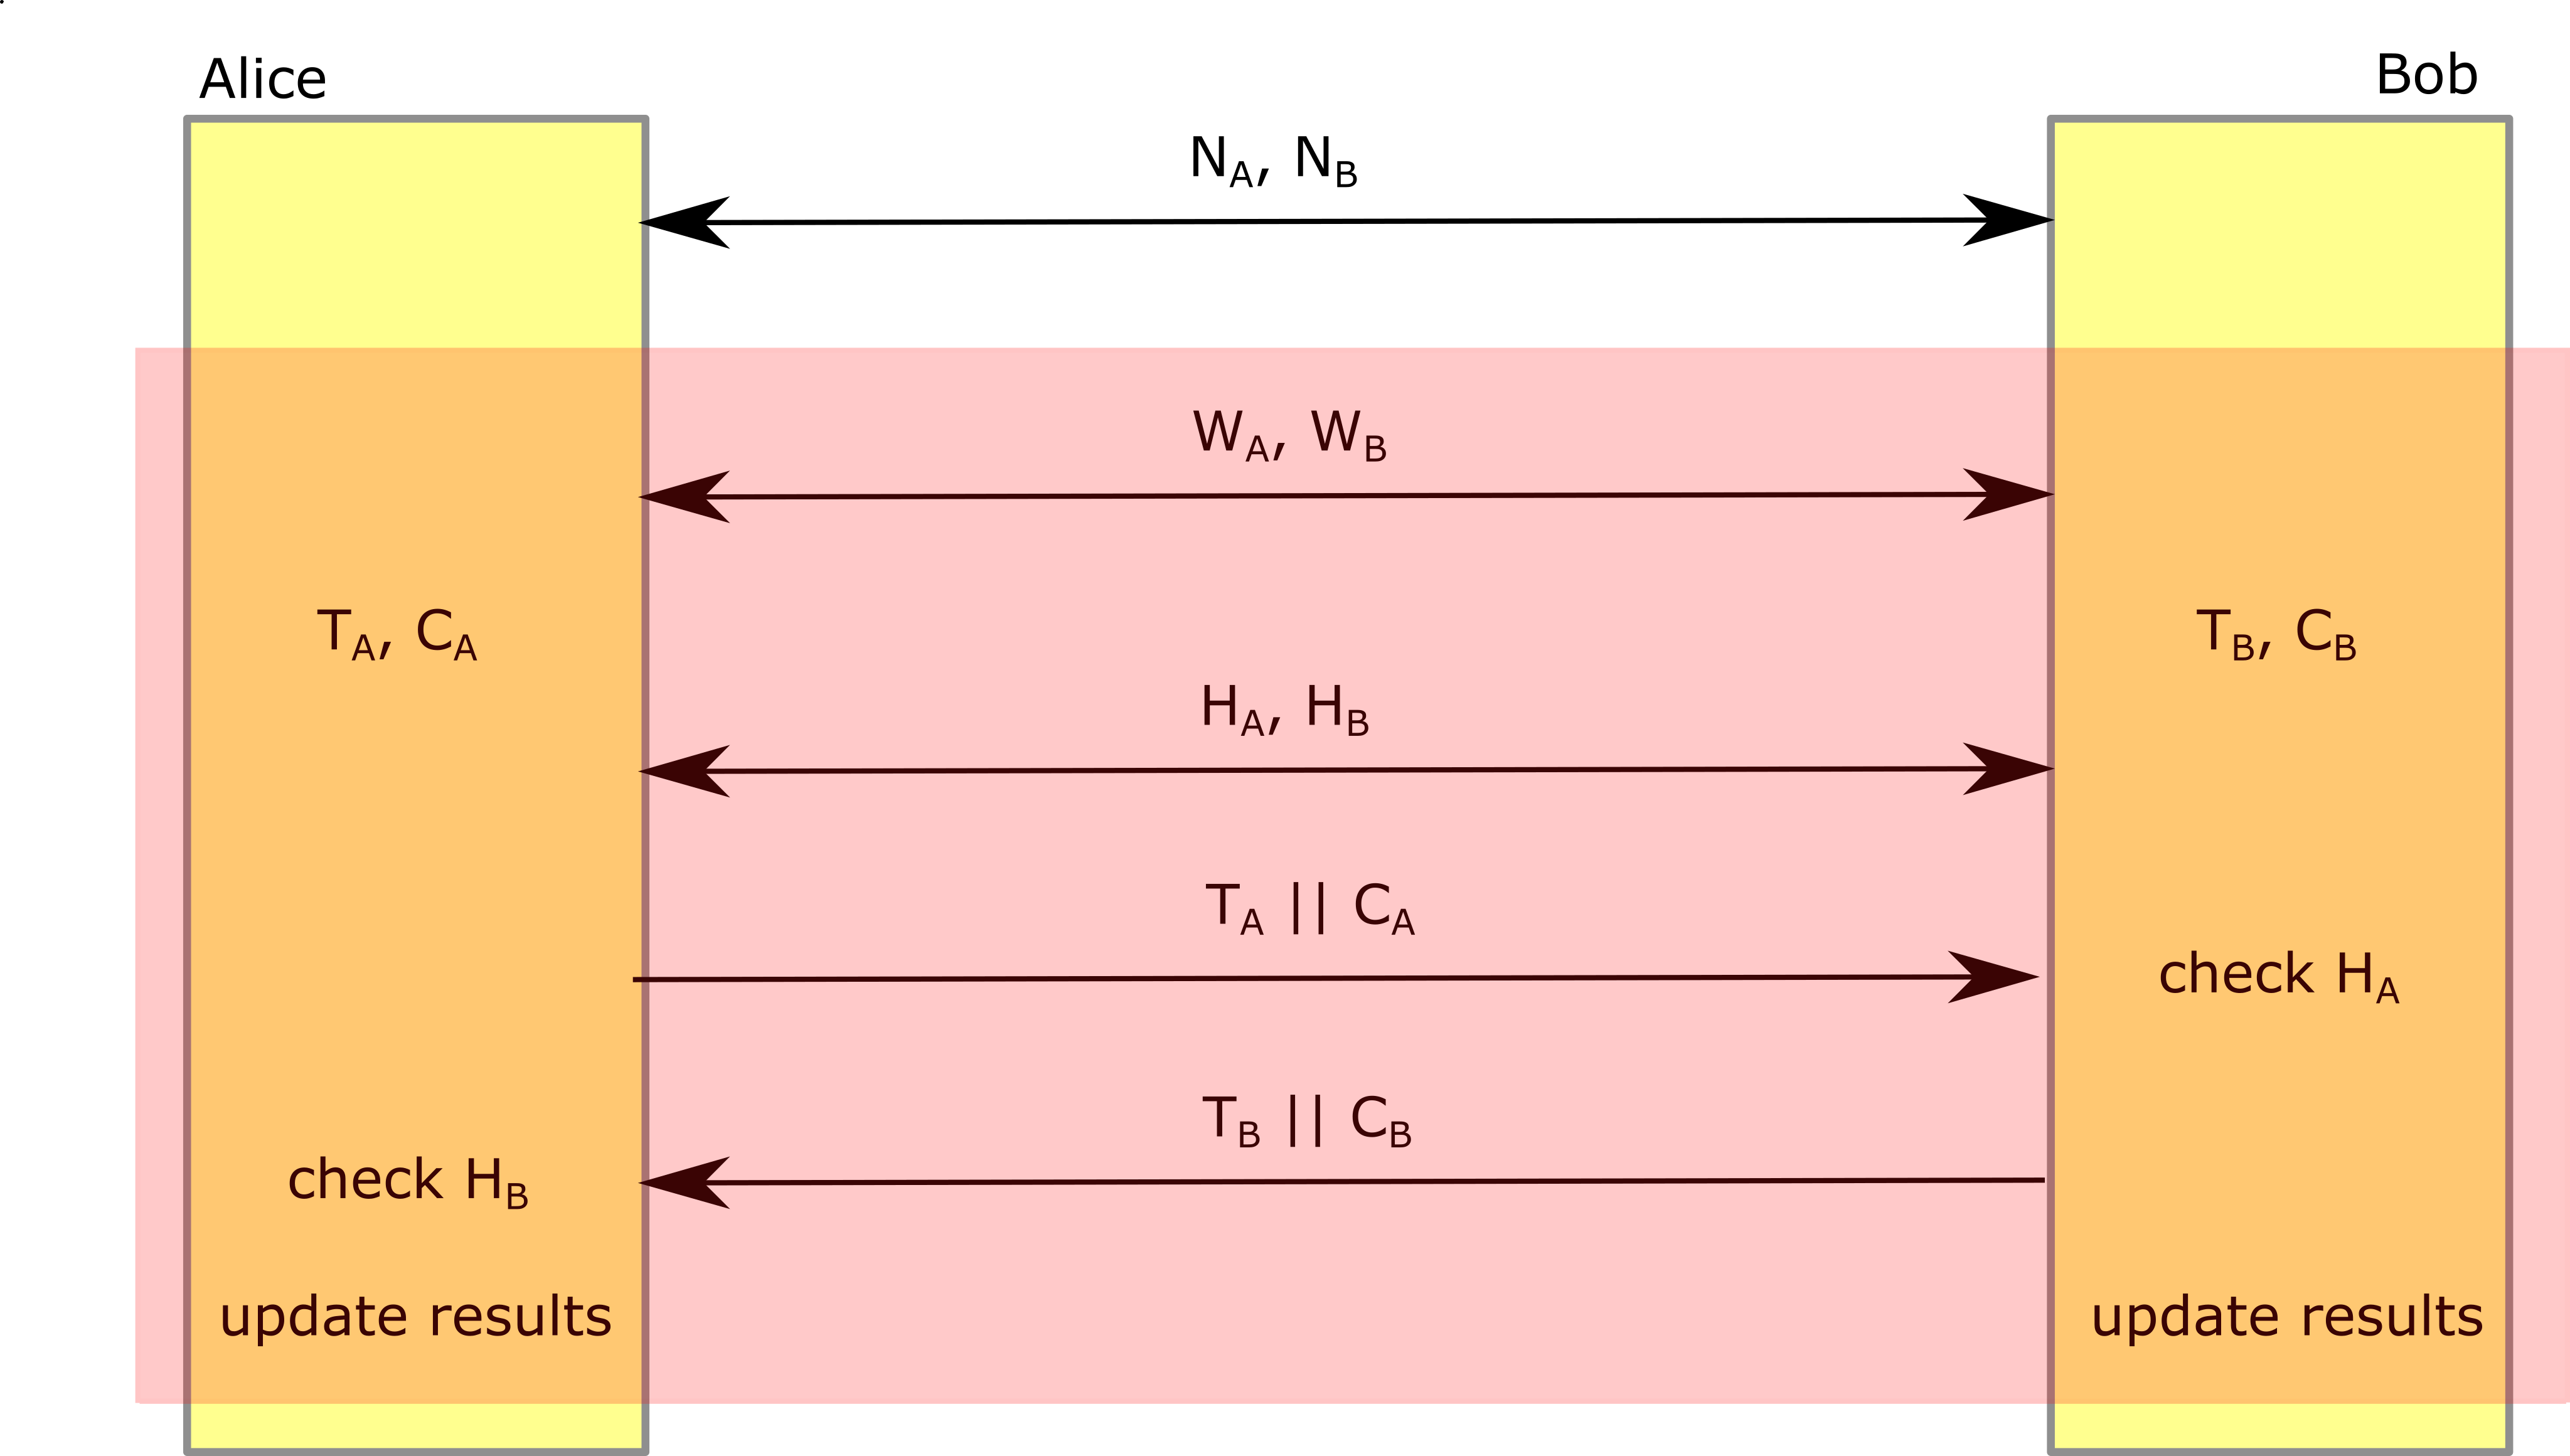
\includegraphics[width=0.8\textwidth]{protocol-hw6-1699981.png} % adjust width
	\caption{\textit{The designed protocol: the loop is inside the red box and terminates when one of the two players wins the match.}} % optional
	\label{fig:protocol}
\end{figure}

\begin{enumerate}
	\item generate nonce (unique per match!)
	\begin{itemize}
		\item Alice sends to Bob a nonce $N_A$
		\item Bob sends to Alice a nonce $N_B$
	\end{itemize}
	\item send match updates
	\begin{itemize}
		\item Alice sends to Bob $(W_A || W_B)$
		\item Bob does the same
		\item they both check if the messages are equal: if not, the opponent is cheating!
	\end{itemize}
	\item check for termination
	\begin{itemize}
		\item if $W_A == p+1$ Alice sends to Bob "I won". Bob checks the value of $W_A$ and replies with a "Congrats".
		\item if $W_B == p+1$ Bob sends to Alice "I won". Alice checks the value of $W_B$ and replies with a "Congrats".
	\end{itemize}
	\item if still playing, generate a nonce (unique per round!)
	\begin{itemize}
		\item Alice generates $T_A$
		\item Bob generates $T_B$
	\end{itemize}
	\item select a choice in ("Paper", "Scissors" ,"Rock")
	\begin{itemize}
		\item Alice selects $C_A$
		\item Bob selects $C_B$
	\end{itemize}
	\item send choices
	\begin{itemize}
		\item Alice sends to Bob $H_A = H( T_A || N_B || C_A )$
		\item Bob sends to Alice $H_B = H( T_B || N_A || C_B )$
	\end{itemize}
	\item reveal choices to the opponent
	\begin{itemize}
		\item Alice sends to Bob $(T_A || C_A)$
		\item Bob sends to Alice $(T_B || C_B)$
	\end{itemize}
	\item check choices
	\begin{itemize}
		\item Alice checks $H_B == H( T_B || N_A || C_B )$
		\item Bob checks $H_A == H( T_A || N_B || C_A )$
	\end{itemize}
	\item update results
	\begin{itemize}
		\item if $C_A > C_B$\footnote{remember that $S > P$, $P > R$ and $R > S$}, increment $W_A$
		\item if $C_B < C_A$, increment $W_B$
	\end{itemize}
	\item repeat from (2)
\end{enumerate}

\subsection{Recap of symbols and acronyms}
\begin{itemize}
	\item H = cryptographic hashing function
	\item $N_A$ = Nonce generated by Alice at the beginning of a match
	\item $N_B$ = Nonce generated by Bob at the beginning of a match
	\item $T_A$ = Nonce generated by Alice, valid for a single round of game
	\item $T_B$ = Nonce generated by Bob, valid for a single round of game
	\item $C_A$ = Choice of Alice
	\item $C_B$ = Choice of Bob
	\item $W_A$ = Number of games won by Alice
	\item $W_B$ = Number of games won by Bob
\end{itemize}

\section{Security}
\subsection{Prevent pre-computations}
The nonces $N_A$ and $N_B$ are useful to prevent computations before the actual match. Without them, a player could prepare a list of pairs (choice, nonce) with colliding hash. Then, once the opponent reveals his choice, he sends back the winning choice and the private nonce values selected from his list.

\subsection{Prevent replay attacks}
The nonces $T_A$ and $T_B$ are needed to prevent replay attacks. If Alice makes a choice $C_A \in \{P, S, R\}$, in the next rounds the same choice leads to a different hash, thus avoiding that Bob knows in advance what is the value chosen.

\subsection{Disputes regarding the winner}
Both Alice and Bob have local counters of the number of games won by them and by their opponent. Before starting a new round of the match, they send each other their local values and compare them: if some value is wrong, it means that one of the players is cheating on the number of won games. It is not possible that Alice and Bob dispute regarding the winner of a game: in fact, once the choices are sent in plaintext together with the private nonce, the two players can compute an hash and compare it with the last message received by the opponent; if one of the two tries to change his choice, the opponent will notice that unfair behavior and quit the game. When one of the two players reaches p + 1 wins, he sends to the opponent a winning message and simply close the connection: the opponent can check if his opponent has won, looking at the number of won games. At this point he simply replies with a congratulations message and close the connection.
\end{document}
